\chapter{Spectral estimation}
\label{app:SpectralEstimation}
In contrast to deterministic processes,
random processes cannot be modeled via an explicit mathematical relationship.
Rather, random processes are characterized
in terms of probabilities and statistical properties.
Any given observation of a random process represents
only one of many possible observations;
each such observation is referred to as
a ``sample'' or a ``realization'' of the random process
and is denoted as $x_k(t)$.
The random process itself consists of
the ensemble of all of the potential observations
and is denoted as $\{x_k(t)\}$.
Random processes can be stationary or nonstationary.
The statistical properties of a stationary random process
do not vary in time, and
the spectral tools discussed below
are all developed for analysis of stationary random processes.


\section{Non-parametric techniques}
\label{app:SpectralEstimation:NonParametric}
Most of the discussion below is distilled from
the seminal work by Bendat and Piersol~\cite{bendat_and_piersol}, and
inquisitive readers are directed there
for a more extensive treatment of the subject.

The windowed, finite Fourier transform $X_k(f, T)$
of a continuous signal $x_k(t)$
sampled for $-T / 2 \leq t < T / 2$
is defined as
\begin{equation}
  X_k(f, T)
  =
  \int_{-T / 2}^{T / 2}
  dt \, [w(t) \cdot x_k(t)] e^{-i \, 2 \pi f t},
  \label{eq:SpectralEstimation:finite_Fourier_transform}
\end{equation}
where $w(t)$ is an arbitrary windowing function.
Typically, the selected windowing function smoothly tapers
as $|t| \rightarrow T / 2$
to minimize sidelobe leakage
that results from discontinuities at the start and end of the sample record.
Further, to prevent power loss, the windowing function
is also typically normalized such that
\begin{equation}
  \frac{1}{T} \int_{-T/2}^{T/2} dt \, [w(t)]^2 = 1.
\end{equation}
The normalized Hanning window is perhaps
the most commonly used windowing function, and
it is used uniformly throughout this work.

For real-valued, stationary random processes $\{x_k(t)\}$ and $\{y_k(t)\}$,
the one-sided \emph{cross-spectral density} function $G_{xy}(f)$ is defined as
\begin{equation}
  G_{xy}(f)
  \equiv
  \lim_{T \rightarrow \infty}
  \frac{2}{T} E \left[ X_k^*(f, T) Y_k(f, T) \right]
  \label{eq:SpectralEstimation:cross_spectral_density_defn}
\end{equation}
for $0 < f < \infty$;
$G_{xy}(f)$ is not defined for $f < 0$, and
it is reduced by a factor of two relative to
(\ref{eq:SpectralEstimation:cross_spectral_density_defn}) at $f = 0$
(the value of $G_{xy}(0)$ is of little relevance to this work).
Note that $E[\cdot]$ is the expectation value operator;
this operator averages over all of the realizations in the ensemble, and
its application ensures that
(\ref{eq:SpectralEstimation:cross_spectral_density_defn})
is a statistically consistent definition of the cross-spectral density
(that is, ensemble averaging is needed for $G_{xy}(f)$
to approach the true cross-spectral density
as $T \rightarrow \infty$). % see pgs. 127, 128 of Bendat & Piersol, 4th ed.
If, in addition to being stationary,
the random process is also \emph{ergodic},
the ensemble average can be replaced
with a time average of $X_k(f, T)$
over successive time slices.
If desired, these time slices may partially overlap.
Unless otherwise noted,
all of the ensemble averages in this work are computed
using this assumption of ergodicity, and
successive slices are selected to overlap by 50\%.

In general $G_{xy}(f)$ is a complex-valued function.
This can be made explicit by writing
\begin{equation}
  G_{xy}(f) = \left| G_{xy}(f) \right| e^{i \alpha_{xy}(f)},
  \label{eq:SpectralEstimation:cross_spectral_density_explicit_complex}
\end{equation}
where $\alpha_{xy}(f)$ is the \emph{cross phase}.
For the special case $\{x_k(t)\} = \{y_k(t)\}$,
$G_{xx}(f)$ is real-valued (i.e.\ $G_{xx}(f) = |G_{xx}(f)|$) and
is referred to as the one-sided \emph{autospectral density} function.

The degree of correlation between random processes
$\{x_k(t)\}$ and $\{y_k(t)\}$ can be easily quantified
with the corresponding spectral density functions.
In particular, the \emph{magnitude-squared coherence} function
$\gamma_{xy}^2(f)$ is defined as
\begin{equation}
  \gamma_{xy}^2(f)
  \equiv
  \frac{|G_{xy}(f)|^2}{G_{xx}(f) G_{yy}(f)},
  \label{eq:SpectralEstimation:magnitude_squared_coherence_defn}
\end{equation}
and it satisfies
\begin{equation}
  0 \leq \gamma_{xy}^2(f) \leq 1
  \label{eq:SpectralEstimation:magnitude_squared_coherence_bounds}
\end{equation}
for $0 \leq f < \infty$.
If $\gamma_{xy}^2(f) = 1$,
$\{x_k(t)\}$ and $\{y_k(t)\}$ are $100\%$ correlated at frequency $f$, and
if $\gamma_{xy}^2(f) = 0$,
$\{x_k(t)\}$ and $\{y_k(t)\}$ are completely uncorrelated at frequency $f$.
Note that the ensemble-averaging operation in
(\ref{eq:SpectralEstimation:cross_spectral_density_defn})
is paramount to the computation
of \emph{informative} values for $\gamma_{xy}^2(f)$;
that is, if ensemble averaging is ignored, and
only single realizations of the random processes are used,
$\gamma_{xy}^2(f) \equiv 1$ for all $f$,
\emph{regardless} of the actual degree of coherence
between between $\{x_k(t)\}$ and $\{y_k(t)\}$.

\begin{table}[t]
  \centering
  \renewcommand{\arraystretch}{1.5}% Spread rows out...
  \begin{tabular}{%
    >{\centering}m{5.0cm} >{\centering}m{5.0cm}
  }
    \toprule%
    \textbf{Spectral estimate}
    & \textbf{Random error} \cite{bendat_and_piersol}
    \tabularnewline%
    \midrule
    $G_{xy}(f)$
    & $\varepsilon \left[G_{xy}(f) \right]
    =
    \frac{1}{|\gamma_{xy}(f)| \sqrt{N_r}}$
    \tabularnewline%
    $\alpha_{xy}(f)$
    & s.d.$\left[ \alpha_{xy}(f) \right]
    \approx
    \frac{[1 - \gamma_{xy}^2(f)]^{1/2}}{|\gamma_{xy}(f)| \sqrt{2 N_r}}$
    \tabularnewline%
    $\gamma_{xy}^2(f)$
    & $\varepsilon \left[ \gamma_{xy}^2(f) \right]
    =
    \frac{\sqrt{2} [1 - \gamma_{xy}^2(f)]}{|\gamma_{xy}(f)| \sqrt{N_r}}$
    \tabularnewline%
    \toprule%
  \end{tabular}
  \caption[Random errors in spectral estimates]{%
    Random errors in estimates of spectral properties are functions of
    the number of realizations $N_r$ used
    in the computation of the ensemble average and
    the coherence magnitude $|\gamma_{xy}(f)|$.
    Here, s.d$[\cdot]$ represents the standard deviation of the estimate, and
    $\varepsilon[\cdot]$ represents the standard deviation of the estimate
    \emph{normalized} to the true value of the spectral property.
    }%
\label{table:ToroidalCorrelation:spectral_estimate_random_errors}
\end{table}

Care should be taken when computing spectral density estimates.
Table~\ref{table:ToroidalCorrelation:spectral_estimate_random_errors}
summarizes the random errors associated with the estimates
of various spectral properties.
Note that the number of realizations $N_r$ used
in the computation of the ensemble average
is a parameter that can be specified
at the time of analysis and that
increasing $N_r$ reduces the random errors of each spectral estimate.
(While increased $\gamma_{xy}^2(f)$ also reduces random errors,
$\gamma_{xy}^2(f)$ is an intrinsic property of the data
rather than a parameter that can be specified at the time of analysis).
Further, in various programming languages,
it is not uncommon to ``detrend'' realizations $x_k(t)$ and $y_k(t)$
by subtracting the signal mean or linear trend
prior to application of
(\ref{eq:SpectralEstimation:cross_spectral_density_defn}).
As described in
Section~\ref{sec:Implementation:DataPreparation:high_pass_filtering},
signals are high-pass filtered prior to spectral analysis, and
no further detrending is performed.


\section{Parametric techniques}
\label{app:SpectralEstimation:Parametric}
Parametric techniques attempt to represent a signal
with a mathematical model containing
a limited number of predefined parameters.
For a pedagogical overview of such techniques,
the reader is directed to
the work of Oppenheim and Schafer~\cite[Ch.~11]{oppenheim}
The discussion here is largely synthesized
from the discussion by Marple~\cite{marple_ieee89}.

Many random processes are well approximated
by rational transfer-function models.
In such models,
an input driving sequence $n_n$ and
an output (i.e. data) sequence $x_n$
are related via the linear difference equation
\begin{equation}
  x_n
  =
  \sum_{l = 0}^q b_l n_{n - l}
  -
  \sum_{k = 1}^p a_k x_{n - k};
  \label{eq:SpectralEstimation:ARMA}
\end{equation}
each sequence has length $N$, and
successive samples are separated in time by $\Delta t$.
Such a model is termed an
autoregressive-moving average (ARMA) model.
Now, if $b_0 = 1$ and the remainder of the $b_l$ are zero,
(\ref{eq:SpectralEstimation:ARMA}) reduces to
\begin{equation}
  x_n
  =
  -\sum_{k = 1}^p a_k x_{n - k}
  +
  n_n
  \label{eq:SpectralEstimation:AR}
\end{equation}
such that $x_n$ is an autoregression of order $p$
driven by white noise $n_n$.
The autospectral density $G_{xx}(f)$ of such an autoregression is
\begin{equation}
  G_{xx}(f)
  =
  \frac{%
    \sigma^2}{%
    \left|
      1
      +
      \sum\limits_{k = 1}^{p} a_k \exp(-2 \pi k f \Delta t)
    \right|^2
  },
  \label{eq:SpectralEstimation:AR_autospectral_density}
\end{equation}
where $\sigma^2$ is the variance of noise term $n_n$.
Because the only frequency dependence in spectral estimate
(\ref{eq:SpectralEstimation:AR_autospectral_density})
appears in the denominator,
the AR model is often referred to as an all-pole model.
In one dimension, AR spectra are equivalent
to spectra computed via the maximum entropy method (MEM).
Interestingly, AR spectra do \emph{not} suffer from
traditional sidelobes due to windowing.

The AR process is fully characterized
by the $(p + 1)$ parameters $(a_1, a_2, \cdots, a_p, \sigma^2)$, and
numerous techniques exist for their estimation.
The $p + 1$ autocorrelations
$\{R_{xx}(0)$, $R_{xx}(\Delta t)$, \ldots $R_{xx}(p \cdot \Delta t)\}$
are related to $(a_1, a_2, \cdots, a_p, \sigma^2)$
via the Yule-Walker normal equations,
which the Levinson-Durbin recursion can efficiently solve
\cite[Sec.~11.6]{oppenheim}.
However, better AR estimates are often obtained
via least-squares linear prediction
applied directly to the data $x_n$.
Such techniques may employ the forward-only linear prediction
or some combination of the forward and reverse linear predictions.
The covariance method~\cite[Sec.~11.3.2]{oppenheim}
is perhaps the most well known forward-only algorithm,
while the Burg method
is perhaps the most well known forward and reverse algorithm.

Here, the Burg method is briefly reviewed.
The algorithm is iterative, so
assume that the $p$\ts{th} order AR parameters are known.
Then, the forward linear prediction is
\begin{equation}
  \hat{x}_n
  =
  -\sum_{k = 1}^p a_{p,k} x_{n - k},
  \label{eq:SpectralEstimation:forward_linear_prediction}
\end{equation}
where $a_{p,k}$ is the $k$\ts{th} coefficient
of the $p$-order AR model.
The corresponding forward linear-prediction error is
\begin{align}
  e_{p,n}
  &=
  x_n - \hat{x}_n
  \notag \\
  &=
  \sum_{k = 0}^p a_{p,k} x_{n - k},
  \qquad
  p \leq n < N,
  \label{eq:SpectralEstimation:forward_linear_prediction_error}
\end{align}
where $a_{p,0} = 1$ by definition and
the limits on $n$ are established
such that the error is defined only over the available data.
Note that $e_{p,n} = n_n$ such that
$\sigma^2 = |e_{p,n}|^2$.
For a stationary process,
the coefficients of the backward linear-prediction error filter
are simply conjugated and reversed in time
relative to those of the forward linear-prediction error filter
such that the backward linear-prediction error is
\begin{equation}
  b_{p,n}
  =
  \sum_{k = 0}^p a_{p,k}^* x_{n - p + k},
  \qquad
  p \leq n < N,
  \label{eq:SpectralEstimation:backward_linear_prediction_error}
\end{equation}
where $z^*$ indicates the complex conjugate of $z$.
The total forward and backward linear-prediction error is
\begin{equation}
  E_p
  =
  \sum_{n = p}^{N - 1} |e_{p,n}|^2
  +
  \sum_{n = p}^{N - 1} |b_{p,n}|^2.
\end{equation}
To estimate the AR parameters,
the Burg method minimizes the total error $E_p$
subject to the constraint that
the AR parameters satisfy the Levinson-Durbin recursion
\begin{equation}
  a_{p,k}
  =
  a_{p - 1, k}
  +
  a_{p,p} a_{p - 1, p - k}^*,
  \qquad
  1 \leq k \leq p.
  \label{eq:SpectralEstimation:Levinson_Durbin_recursion}
\end{equation}
The Levinson-Durbin constraint
ensures that the AR filter is stable
(i.e.\ all poles fall within the unit circle) and
make $E_p$ a function solely of the unknown coefficient $a_{p,p}$.
Setting the derivative of $E_p$
with respect to $a_{p,p}$ to zero then yields
\begin{equation}
  a_{i,i}
  =
  \frac{%
    -2 \sum\limits_{k = i}^{N - 1}
    b_{i - 1, k - 1}^*
    e_{i - 1, k}
  }{%
    \sum\limits_{k = i}^{N - 1}
    \left(%
      |b_{i - 1, k - 1}|^2
      +
      |e_{i - 1, k - 1}|^2
    \right)
  }.
  \label{eq:SpectralEstimation:a_ii}
\end{equation}

Although the Burg method has satisfactory performance for the present work,
it should be noted for completeness that
the Burg method suffers from several problems,
including spectral line splitting and biases in the frequency estimate.
These problems can be corrected via
a ``least-squares'' algorithm
(independently developed by Ulrych-Clayton and Nuttall)
in which $E_p$ is differentiated with respect to all of the $a_{p,k}$,
not just $a_{p,p}$,
to obtain a set of normal equations
(the Levinson-Durbin constraint is no longer enforced).
Application of this modified algorithm
is relegated to future work.


\section{Hybrid two-dimensional spectral estimates}
\label{app:SpectralEstimation:2d_spectra}
\begin{figure}
  \centering
  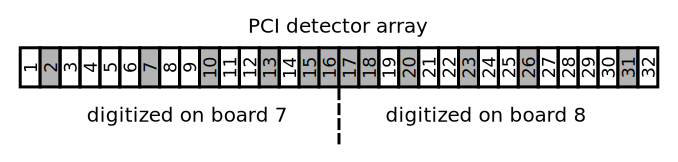
\includegraphics[width = \textwidth]{%
    Appendices/SpectralEstimation/figs/pci_detector_array.pdf}
  \caption[Schematic of PCI detector array]{%
    Schematic of PCI detector array.
    Only the gray channels are digitized.
  }
  \label{fig:SpectralEstimation:pci_detector_array}
\end{figure}

The PCI detector consists of $32$ elements arranged in a linear array.
However, due to digitization constraints,
only a subset of the signals from the linear array are digitized.
Further, to achieve reasonable mid-$k$ and high-$k$ response,
this subset of channels is non-uniformly spaced, as indicated in
Figure~\ref{fig:SpectralEstimation:pci_detector_array}.
This immediately precludes direct application
of the fast Fourier transform (FFT) in the spatial dimension, and
more elaborate schemes must be utilized
to quantify the spatial spectrum.
Below, Section~\ref{app:SpectralEstimation:2d_spectra:trigger_offset}
describes the estimation and compensation
of the trigger offset between the two PCI digitizer boards.
Then, Section~\ref{app:SpectralEstimation:2d_spectra:correlation_function}
discusses estimation of the two-dimensional autocorrelation function,
which can be computed even when channels are non-uniformly spaced.
Finally, Section~\ref{app:SpectralEstimation:2d_spectra:2d_spectra}
discusses calculation of the two-dimensional autospectral density
from the two-dimensional autocorrelation function.


\subsection{Estimation \& compensation of trigger offset}
\label{app:SpectralEstimation:2d_spectra:trigger_offset}
Prior to performing any spectral computations,
the trigger offset between
digitizer board $7$ and digitizer board $8$
must be estimated and compensated.
The general theory is discussed in
Appendix~\ref{app:DigitizerSynchronization}.
The trigger offset is estimated by defining
\begin{align}
  \Delta \alpha(f)
  &=
  \frac{\alpha_{15,16}(f) + \alpha_{17,18}(f)}{2}
  \\
  \Delta \alpha_{\meas}(f)
  &=
  \alpha_{16,17}(f),
\end{align}
and applying
(\ref{eq:DigitizerSynchronization:trigger_offset_estimate_apriori_phase});
here $\alpha_{i,j}(f)$ is the cross phase
between channels $i$ and $j$
during a stationary portion of the discharge.
To minimize random error,
at least $1000$ realizations are averaged over, and
only frequencies with sufficiently high coherence
(e.g.\ $\gamma^2_{i,j} \geq 0.1$) are considered.
The offset is rarely larger than one or two timestamps, but
even such small offsets can significantly bias spectral estimates.
Then, using standard techniques~\cite[Sec.~4.5]{oppenheim},
the trigger offset can be compensated easily in post-processing,
even if the offset is a non-integer multiple of the sample spacing.


\subsection{Two-dimensional autocorrelation function}
The autocorrelation function $R_{x}$ and
the autospectral density function $S_{x}$
are Fourier transform pairs, i.e.\
\begin{align}
  S_{x}(\xi, f)
  &=
  \mathcal{F}[R_{x}(\delta, \tau)](\xi, f),
  \label{eq:SpectralEstimation:autospectral_density_from_autocorrelation}
  \\
  R_{x}(\delta, \tau)
  &=
  \mathcal{F}^{-1}[S_{x}(\xi, f)](\delta, \tau),
  \label{eq:SpectralEstimation:autocorrelation_from_autospectral_density}
\end{align}
where
$\mathcal{F}$ is the Fourier transform,
$\tau$ is the temporal lag,
$\delta$ is the spatial lag,
$f$ is the frequency, and
$\xi$ is the spatial frequency
(related to the wavenumber $k$ via $k = 2 \pi \xi$).
If the measurements are uniformly sampled in space and time,
it is most efficient to estimate
the two-dimensional autospectral density $S_{xx}$
using the FFT methods described in
Section~\ref{app:SpectralEstimation:NonParametric} and
then apply the inverse Fourier transform
as in (\ref{eq:SpectralEstimation:autocorrelation_from_autospectral_density})
to compute the two-dimensional autocorrelation function $R_{x}$.
However, if the measurements are \emph{not} uniformly spaced,
the two dimensional autocorrelation function
can still be estimated via the definition
\begin{equation}
  R_{x}(\delta, \tau)
  =
  E[x_k(z, t) \cdot x_k(z + \delta, t + \tau)],
  \label{eq:SpectralEstimation:autocorrelation_definition}
\end{equation}
where $E[\cdot]$ is the expectation-value operator and
$x_k$ is the $k$\ts{th} realization
of the real-valued random process $\{x_k(z, t)\}$.
If needed, the autocorrelation can be interpolated onto a uniform grid, and
the autospectral density $S_{x}$ can be computed
by applying the Fourier transform,
as in (\ref{eq:SpectralEstimation:autospectral_density_from_autocorrelation}).

When temporal sampling is uniform but spatial sampling is nonuniform,
as in the PCI,
it is often convenient to define a
``hybrid'' two-dimensional autocorrelation function $\tilde{R}_x$
\begin{align}
  \tilde{R}_{x}(\delta, f)
  &=
  \mathcal{F}^{-1}[S_{x}(\xi, f)](\delta)
  \notag \\
  &=
  \int_{-\infty}^{\infty}
  d\xi e^{i 2 \pi \xi \delta}
  S_{x}(\xi, f)
  \notag \\
  &=
  S_{x}(\delta, f),
\end{align}
where $S_x(\delta, f) = S_{x_i, x_j}(f)$ with $i - j = \delta$
is the cross-spectral density function
between $x_i(t) = x(z, t)$ and $x_j(t) = x(z + \delta, t)$.
Note that $S_{x_i, x_j}(f)$ can be efficiently estimated
via the FFT methods described in
Section~\ref{app:SpectralEstimation:NonParametric}
such that the ``hybrid'' autocorrelation function can be estimated as
an ensemble average over all of the unique correlation pairs
separated by $\delta$
\begin{equation}
  \tilde{R}_{x}(\delta, f)
  =
  \frac{%
    \sum\limits_{i - j = \delta} S_{x_i, x_j}(f)
  }{%
    \sum\limits_{i - j = \delta} 1
  };
  \label{eq:SpectralEstimation:hybrid_autocorrelation_estimate}
\end{equation}
if there are no correlation pairs separated by $\delta$,
then $\tilde{R}_x$ is undefined for this separation.
If the variances of $x_i$ and $x_j$ are artificially biased
e.g.\ due to the finite PCI beam width,
the variances should be equalized prior to estimating $\tilde{R}_x$ with
(\ref{eq:SpectralEstimation:hybrid_autocorrelation_estimate}).
As discussed in Section~\ref{app:SpectralEstimation:2d_spectra:2d_spectra},
the autospectral density can be computed
from this $\tilde{R}_x$ estimate.

Before proceeding, however, it is instructive
to consider a few properties of $\tilde{R}_x$.
In general, $\tilde{R}_x$ is complex-valued.
For real-valued $x$, however,
$\tilde{R}_x$ is Hermitian,
i.e.\ $\tilde{R}_x(-\delta, -f) = [\tilde{R}_x(\delta, f)]^*$,
where $z^*$ indicates the complex conjugate of $z$.
At any given frequency $f$,
$\tilde{R}_x(\delta, f)$ attains a maximum at $\tilde{R}_x(0, f)$.
The variance of signal $x(z, t)$ is related to $\tilde{R}_x$ via
\begin{equation}
  \text{var}(x)
  =
  \int \tilde{R}_x(0, f) df.
\end{equation}
Because $|\tilde{R}_x|$ can vary by several orders of magnitude
across the full temporal bandwidth of signal $x(z, t)$,
visualizing the spatiotemporal structure of $\tilde{R}_x$
can be aided by defining the normalized autocorrelation function
\begin{equation}
  \tilde{r}_x(\delta, f)
  =
  \frac{\tilde{R}_x(\delta, f)}{\tilde{R}_x(0, f)}.
\end{equation}
An example of the PCI-measured $\tilde{r}_x(\delta, f)$ is shown in
Figure~\ref{fig:SpectralEstimation:corr_example}.

\label{app:SpectralEstimation:2d_spectra:correlation_function}
\begin{figure}
  \centering
  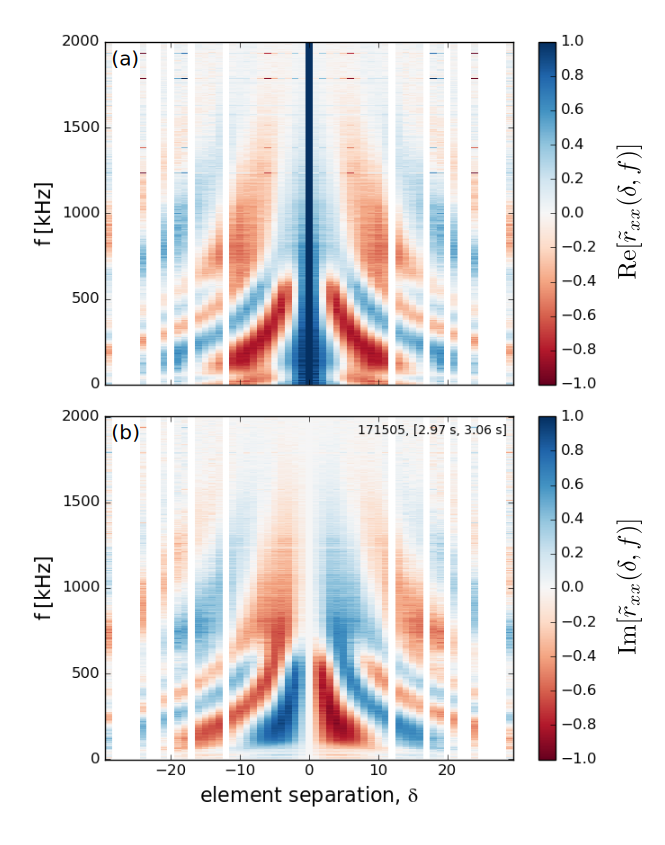
\includegraphics[width = 0.75 \textwidth]{%
    Appendices/SpectralEstimation/figs/corr_example.png}
  \caption[Normalized, $2$d, hybrid autocorrelation function]{%
    Example of the (a) real and (b) imaginary components
    of the PCI-measured normalized, two-dimensional, hybrid
    autocorrelation function $\tilde{r}_x(\delta, f)$.
    Note that $\delta = 0$ corresponds to the same detector element,
    $\delta = 1$ corresponds to adjacent detector elements, etc.
    The vertical white striations correspond to
    non-existing element separations
    (as established by the digitization layout shown in
    Figure~\ref{fig:SpectralEstimation:pci_detector_array})
    for which $\tilde{r}_x(\delta, f)$ is not defined.
    To proceed with the autospectral density estimation
    in Section~\ref{app:SpectralEstimation:2d_spectra:2d_spectra},
    the computation must either be restricted
    to the central, continuous domain, or
    the autocorrelation function must be interpolated;
    linear interpolation was found to be sufficient in this work.
  }
  \label{fig:SpectralEstimation:corr_example}
\end{figure}


\subsection{Two-dimensional autospectral density}
\label{app:SpectralEstimation:2d_spectra:2d_spectra}
\begin{figure}
  \centering
  \includegraphics[width = 0.75 \textwidth]{%
    Appendices/SpectralEstimation/figs/Skf_example.png}
  \caption[$2d$ autospectral density estimates]{%
    $2d$ autospectral density estimates.
  }
  \label{fig:SpectralEstimation:Skf_example}
\end{figure}


\bibliographystyle{plainurl}
\bibliography{references}
